\documentclass[11pt]{opticajnl}
\journal{opticajournal} % use for journal or Optica Open submissions

% See template introduction for guidance on setting shortarticle option
\setboolean{shortarticle}{true}
% true = letter/tutorial
% false = research/review article

% ONLY applicable for journal submission shortarticle types:
% When \setboolean{shortarticle}{true}
% then \setboolean{memo}{true} will print "Memorandum" on title page header
% Otherwise header will remain as "Letter"
% \setboolean{memo}{true}


\usepackage{lineno}
\usepackage{listings}
\usepackage{multicol}

%\linenumbers % Turn off line numbering for Optica Open preprint submissions.

\title{Método de descenso de gradiente en regresión}

\author[1,2,3]{Luis Ardévol Mesa}


\begin{abstract}
Se tratará de resolver un problema de regresión con el método de descenso de gradiente (GD). Se escogerá un problema para el cuál la solución óptima se pueda conseguir con la función \textit{lm} de \textit{R}, permitiendo así hacer una comparativa de los resultados.
\end{abstract}

\setboolean{displaycopyright}{false} % Do not include copyright or licensing information in submission.

\begin{document}

\maketitle

Con el fin de facilitar la escalabilidad del programa, el código se fragmentó en funciones: una para definir el problema, otra para la función de coste y otra para el propio algoritmo del descenso de gradiente. De este modo, si se quiere cambiar el problema o la función de coste, solo hay que declarar/modificar una función, no es necesario modificar el propio algoritmo.

\section{Definición del problema}

Se estudiarán dos modelos de regresión distintos, un modelo multilineal general de $p$ coeficientes y un modelo cuadrático simple, de tres coeficientes. Para el primero, se mostrarán los resultados tanto para el caso particular de un modelo de regresión lineal simple ($p = 1$) como para un número mayor de predictores (concretamente, tomaremos $p = 10$). Las muestras de los predictores se generarán en ambos casos a partir de una distribución uniforme, y se dividirán $X$ e $Y$ en conjuntos de entrenamiento (75\%) y \textit{test} (25\%). \\

\noindent Un modelo de regresión multilineal general tiene la forma: 
\begin{equation}
Y = \beta_0 + \beta_1X_1 + \beta_2X_2 + \cdots + \beta_pX_p + \epsilon 
\end{equation}

\noindent y, fijando $p=1$, se obtiene el modelo lineal simple:
\begin{equation}
Y = \beta_0 + \beta_1X_1 + \epsilon 
\end{equation}

\noindent donde $\epsilon$ es un término de error generado a partir de una distribución normal de media 0 y varianza 1 (si bien se pueden cambiar, los resultados de este ejercicio mantienen estos valores constantes en todos los modelos considerados). \\

\noindent El problema cuadrático se expresa de la siguiente forma:
\begin{equation}
    Y = \beta_0 + \beta_1 X_1 + \beta_2 X_2^2 + \epsilon
\end{equation}

\noindent siendo $\epsilon$ un término de error de la misma naturaleza que el descrito antes. \\

Por tanto, en general se tendrá una matriz $X$ de dimensión $n\times p+1$ (donde la primera columna es de 1, actuando como la identidad), $\beta$ un vector de $p+1$ valores y $\epsilon$ un vector de $n$ valores. Así, la respuesta $Y$ será un vector de $n$ valores generado como
\begin{equation}
Y = X \cdot \beta + \epsilon
\end{equation}

Pese a que una función hubiese sido suficiente para definir ambos problemas, se declaran en funciones separadas para mostrar la escalabilidad del código.

\section{Función de coste}

La función de coste o pérdida será la función a minimizar durante el descenso de gradiente. Existen multitud de opciones, y se suele elegir a partir de la distribución de los datos. Por ejemplo, la precipitación acumulada puede seguir una distribución Bernouilli-Gamma, de modo que una opción para hacer predicciones sobre esta variable es minimizar la verosimilitud logarítmica negativa de esa distribución (\textit{negative log-likelihood}). Sin embargo, hay funciones de coste que, aunque no sean las más adecuadas para todas las distribuciones de datos, son usadas en multitud de problemas debido a su buen rendimiento general y su fácil interpretación, entre otros motivos. \\

En este caso, al tener distribuciones uniformes, implementaremos dos funciones de coste muy similares: la suma de los residuos al cuadrado (RSS), que es la función a minimizar estándar en problemas lineales,

\begin{equation}
RSS(\beta_0, \beta_1, \dots, \beta_p) = \sum_{i=1}^n (y_i - \beta_0 - \beta_1 x_{i1} - \dots - \beta_p x_{ip})^2
\end{equation}

\noindent y el error cuadrático medio, otro estándar que simplemente normaliza el error total, facilitando la interpretabilidad (al tratarse de la media del error de una observación) y escalabilidad,
\begin{equation}
MSE(\beta_0, \beta_1, \dots, \beta_p) = \frac{1}{n}\sum_{i=1}^n (y_i - \beta_0 - \beta_1 x_{i1} - \dots - \beta_p x_{ip})^2
\end{equation}

De nuevo, cada una de estas será una función diferente en nuestro código, que se pasará como argumento a la función que aplique el algoritmo de descenso de gradiente. 


\section{Descenso de gradiente}

Sea un punto inicial $x \in \text{dom}f$, se determina la dirección de descenso $\Delta x = -\nabla f(x)$ y, con un paso de tamaño $t > 0$, se actualiza el valor de $x$ de forma que 
\begin{equation}
x := x + t\Delta x
\end{equation}

Este proceso se repite de forma iterativa hasta cumplir un criterio de parada, que en este caso fijaremos en $||\nabla f(x)||^2 \leq \text{tol}$, donde tol es una tolerancia (valor usualmente pequeño, que tomaremos por defecto como $10^{-5}$). 

El algoritmo de descenso de gradiente puede tener paso fijo, usar \textit{exact line search}, es decir, buscar el paso óptimo en cada iteración, o usar \textit{backtracking line search}, para buscar el paso óptimo de una forma más ligera computacionalmente, pero menos precisa. En este caso, programaremos el algoritmo para usar paso fijo (\texttt{usebacktracking = FALSE}) y para usar \textit{backtracking line search} (\texttt{usebacktracking = TRUE}). \\

Este último método de buscar el paso lo podemos resumir como sigue: sea una dirección de descenso $\Delta x$ para un $f$ en $x \in \text{dom}(f)$, $\alpha \in (0, 0.5]$ y $\beta \in (0, 1)$, con $t:= 1$, mientras $f(x + t\Delta x) > f(x) + \alpha t \nabla f(x)^T\Delta x$, se hace $t := \beta t$. \\

Usar $x$ como punto general no es más que una notación. Hay que tener muy en cuenta que, en este caso, se buscan los coeficientes $\beta_i$, es decir, la función a minimizar depende de $f = f(\beta_0, \beta_1, \dots, \beta_p)$, el gradiente son derivadas respecto a estos $\beta$, etc. En la función que implementa este algoritmo, se dejan como parámetros opcionales el paso fijo $t$, el número máximo de iteraciones, la tolerancia y los valores de beta iniciales. La función de pérdida por defecto será la RSS, pero se puede cambiar. En caso de alcanzar el máximo de iteraciones, se devolverá el valor actual junto con un aviso de que no se alcanzó la convergencia. Además, otro parámetro opcional permite alternar entre el uso de paso fijo o \textit{backtracking}. El uso de ambos se comparará en los resultados. \\

Si se toma un paso fijo, hay que evitar coger un paso muy grande, para no caer en oscilaciones o divergencias, o uno muy pequeño, que no llegará al mínimo que buscamos. Como la búsqueda de un paso óptimo puede ser una tarea repetitiva, se hace una función adicional que comprueba los resultados de las estimaciones sobre un conjunto de valores de $t$ dado, devolviendo el mejor resutado junto con el paso del mismo. Además, en cada iteración calcula el resultado usando las dos funciones de pérdida declaradas anteriormente, quedándose con el mejor resultado y mostrando por pantalla que función de coste usó para obtenerlo. En caso de dar ambas el mismo resultado (lo que ocurrirá con estas dos elecciones), también lo mostrará por pantalla. Aquí se entiende por mejor resultado el más próximo a los valores dados por el método \texttt{lm()} para el mismo problema. \\

Las cota superior al valor de $t$ se buscó para ser la mayor posible sin generar divergencias, mientras que para la cota inferior se buscó un compromiso entre alcanzar una solución adecuada y el número de iteraciones máximo. 

\section{Resultados}

Una variable de interés en cualquier algorítmo de optimización o aprendizaje estadístico es la pérdida. Permite evaluar la convergencia y el rendimiento del modelo, así como un posible \textit{overfitting} o \textit{underfitting}. Una representación de la evolución de esta variable con cada iteración resulta útil y necesaria en muchos casos. Aquí, se mostrará esta curva junto a un zoom de la misma, para visualizar la convergencia de forma más clara. \\

Al hacer predicciones y conocer los resultados esperados, siempre es interesante ver cómo de próximas son estas predicciones a los datos reales u observados. Numéricamente, esto se podría cuantificar de diversas formas, pero aquí se mostrará una representación visual. Si se representan los valores predichos frente a los observados, el caso ideal sería que los puntos se situaran sobre la recta de pendiente unidad $y = x$. \\

El objetivo final de este ejercicio es la estimación de los coeficientes del modelo de regresión usado. Se necesita conocer las estimaciones hechas por descenso de gradiente (GD) y los valores calculados a partir del método \texttt{lm()}. Para ver la similitud entre ambos resultados, se mostrarán los valores numéricos exactos en una tabla y se acompañará de una representación visual:
\begin{itemize}
\item Para un número bajo de predictores, es decir, para el caso del modelo lineal simple y el modelo cuadrático ($p = 1$ y $p = 2$ respectivamente), se usará un gráfico de barras que ayude a la comparación de los coeficientes a partir de GD con paso fijo, GD con \textit{backtracking} y \texttt{lm()}. 
\item Para un número alto de predictores, como $p = 10$, la representación anterior no es del todo óptima. Para estos casos, una aproximación similar a la hecha para comparar los resultados predichos y observados resulta conveniente: se representarán los coeficientes estimados por GD frente a los dados por \texttt{lm()} y, en el caso ideal, deberían caer todos sobre la recta $y = x$.
\end{itemize}

\noindent Para el GD con \textit{backtracking} se probó con varios valores de $t$ iniciales, se muestran los mejores resultados. 

\subsection{Modelo de regresión lineal simple}

\subsubsection{Entrenamiento}

\begin{table}[h]
    \centering
    \begin{tabular}{ccc}
    \hline
    \textbf{Método} & \textbf{Intercepto} & \textbf{Pendiente} \\
    \hline
    Coeficientes GD (paso fijo) & $0.5541949$ & $1.5978487$ \\
    Coeficientes GD (backtracking) & $0.5527288$ & $1.5978977$ \\
    Coeficientes lm & $0.5542852$ & $1.5978982$ \\
    \hline
    \end{tabular}
    \caption{Coeficientes estimados para el modelo de regresión lineal simple durante el entrenamiento.}
    \label{tab:mrs}
\end{table}

En la tabla \ref{tab:mrs} se muestran los coeficientes estimados por GD para este modelo. En este caso, el mejor resultado con un paso fijo se obtiene fijando un $t=0.03$ y converge en apenas 105 iteraciones, resultando valores muy próximos a los dados por \texttt{lm()}. El caso de \textit{backtracking} tarda menos en converger y da un intercepto menos acertado, pero una pendiente más próxima al valor esperado. Al tratarse de un modelo tan simple, usar un paso fijo resulta una forma eficiente de llegar a la mejor estimación posible. \\

\noindent A continuación, en la figura \ref{fig:1} se muestran los resultados de este modelo de forma gráfica.

\begin{figure}[H]
\centering
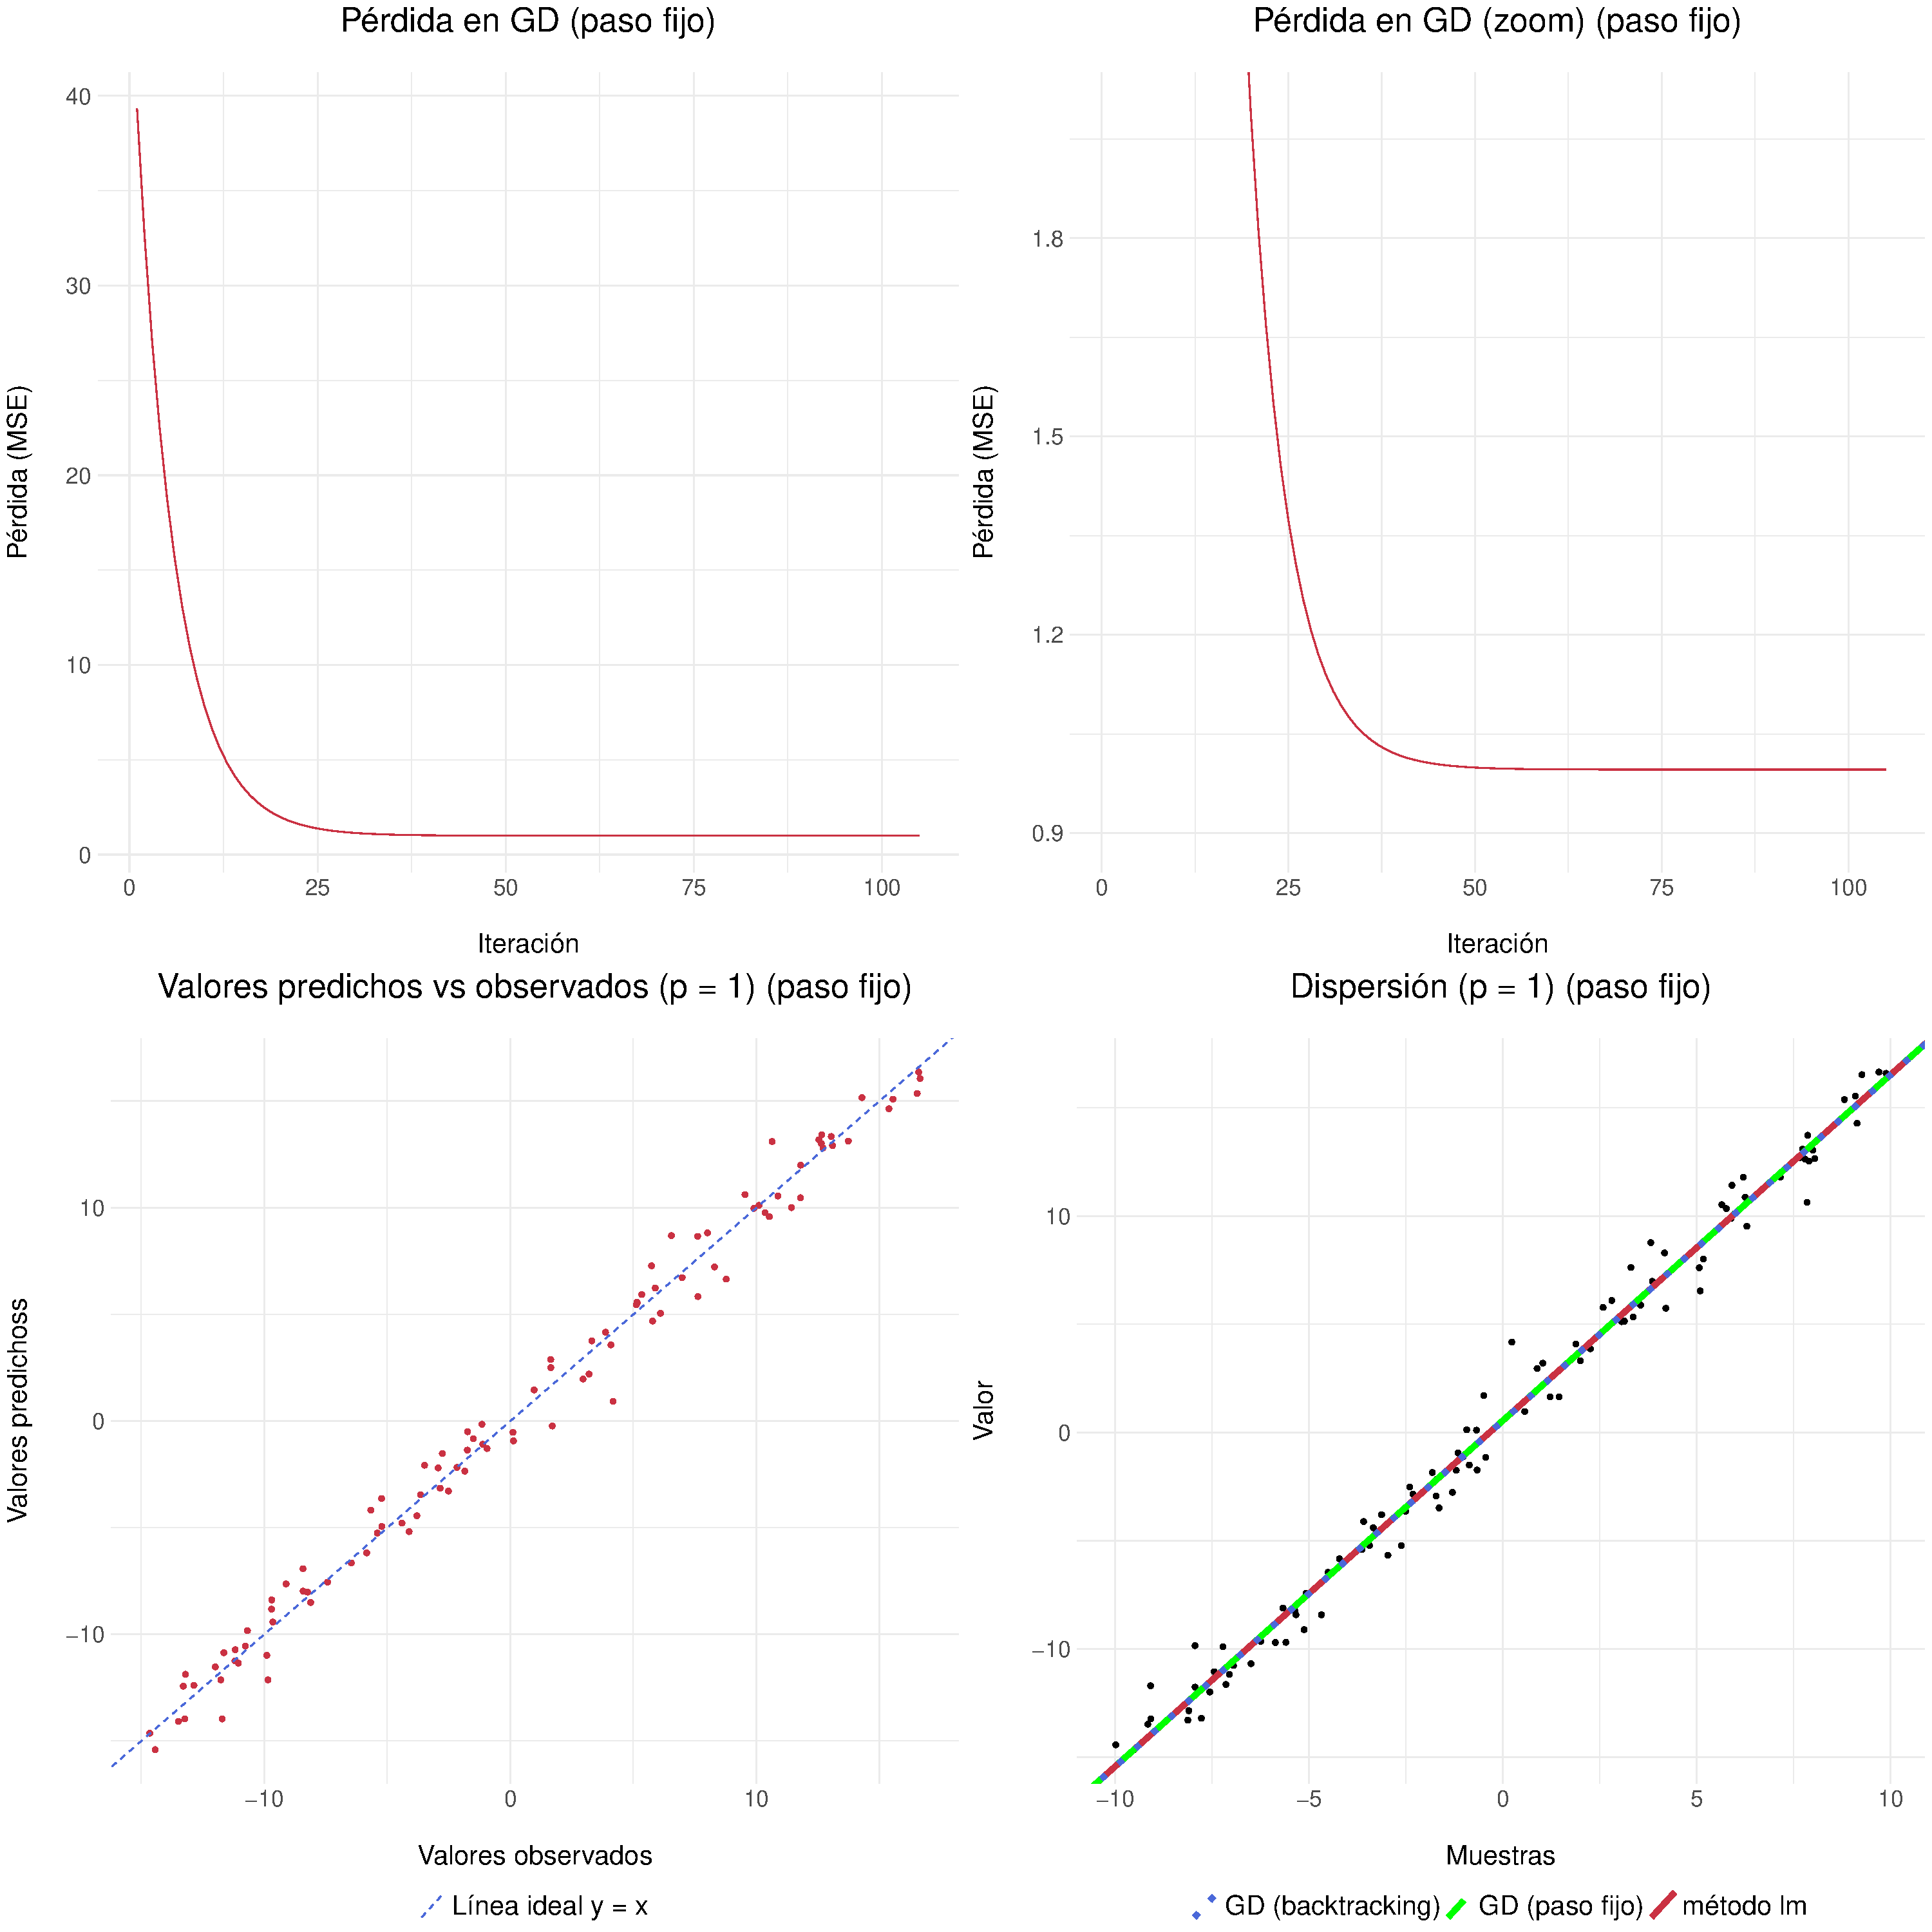
\includegraphics[width=\textwidth]{fotos/plotmrs.pdf}
\end{figure}

\begin{figure}[H]
\centering
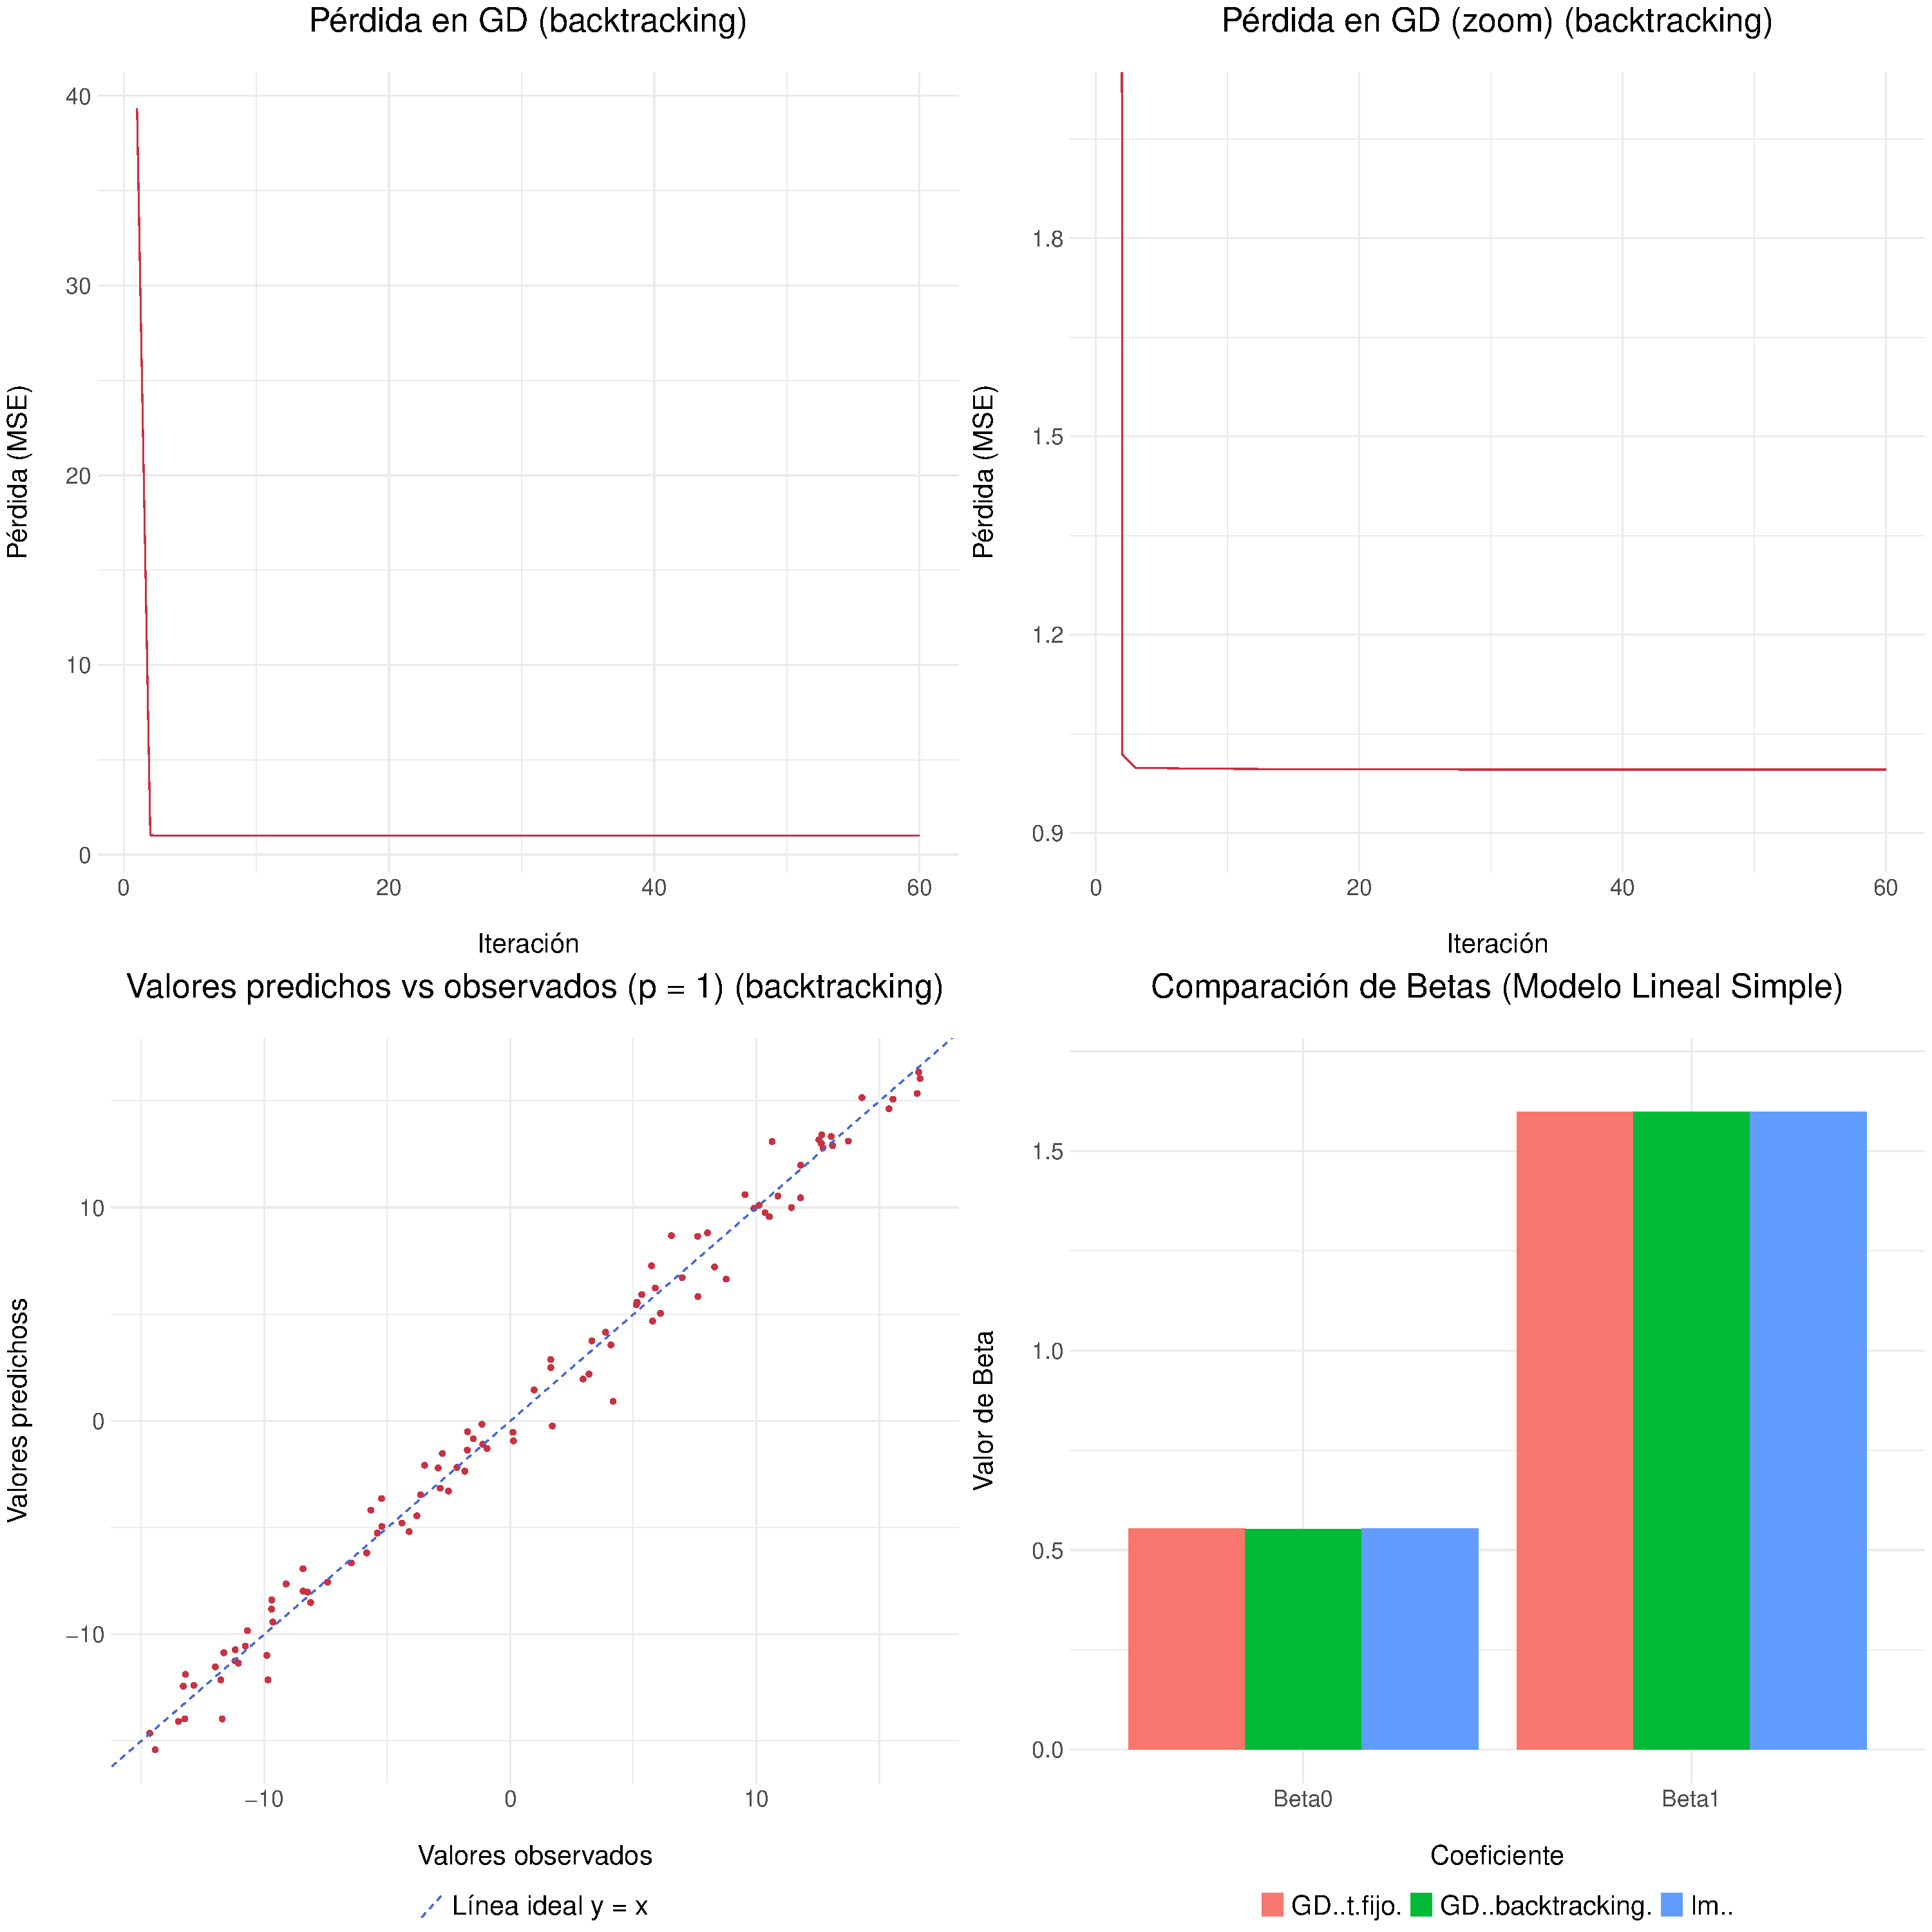
\includegraphics[width=\textwidth]{fotos/plotmrsback.pdf}
\caption{Resultados de entrenamiento del modelo lineal simple haciendo uso de paso fijo y \textit{backtracking}, empleando MSE como función de coste.}
\label{fig:1}
\end{figure}


La primera diferencia apreciable se ve en la evolución de la pérdida y el número de iteraciones. Para un paso fijo, variando el tamaño del paso en tres ordenes de magnitud, se llega a la conclusión de que el mejor resultado se obtiene con un $t = 0.03$, como ya comentamos. Este paso es relativamente grande, y sirve como punto de partida al \textit{backtracking}, que variando el paso a partir de dicho valor consigue converger en la mitad de iteraciones. Para el primer caso, se tiene una curva suave, mientras que con el \textit{backtracking} se tiene una curva mucho más acusada. \\

No hay una diferencia apreciable en los valores predichos por ambos métodos y los dados por \texttt{lm()}. Esto era de esperar, ya que los valores numéricos de los coeficientes comienzan a diferir, como muy pronto, en la tercera cifra decimal. Si se supone que la recta de ajuste es la ideal, $y = x$, se puede estimar la desviación respecto de esta con una estadística $R^2$ y el RSE:
\begin{multicols}{2} 
\begin{itemize}
\item RSE paso fijo: $1.003051$ 
\item $R^2$ paso fijo: $0.9878813$ 
\item RSE \textit{backtracking}: $1.003052$
\item $R^2$ \textit{backtracking}: $0.9878813$
\end{itemize}
\end{multicols}

En ambos casos, tenemos un $R^2$ muy cercano a uno, lo que sugiere que la mayor parte de la variabilidad de los datos queda recogida por la recta ideal a la que deberían ajustarse. Además, el RSE de $1.00$, siendo que los valores observados y predichos se mueven en un rango aproximado $[-15, 15]$, indica poca dispersión de los datos. Visualmente, se comprobó que las predicciones eran similares a los valores observados, ya que los puntos caen muy próximos a la recta ideal, pero con este breve análisis numérico se verifica esto de forma más rigurosa. \\

Otra representación que se muestra es una gráfico de dispersión de los valores de y reales frentre a las muestras $X$. Sobre este, se pintan las tres rectas de ajuste: GD con paso fijo y \textit{backtracking}, y con \texttt{lm()}. De nuevo, por la similitud de los coeficientes, estas tres rectas son casi idénticas y se solapan. A simple vista, resultan un buen ajuste y, numéricamente, se demuestra que es un resultado muy acertado:
\begin{multicols}{2}
\begin{itemize}
\item RSE paso fijo: $1.008156$ 
\item $R^2$ paso fijo: $0.9878813$ 
\item RSE \textit{backtracking}: $1.008157$
\item $R^2$ \textit{backtracking}: $0.9878813$
\end{itemize}
\end{multicols}

Para terminar, se muestra un gráfico de barras con la información vista en la tabla \ref{tab:mrs}. No hay nada nuevo que comentar respecto al mismo, simplemente es una alternativa cómoda para la comparación de los valores de un forma menos precisa que la numérica. 

\subsubsection{Predicciones}

\begin{figure}[H]
\centering
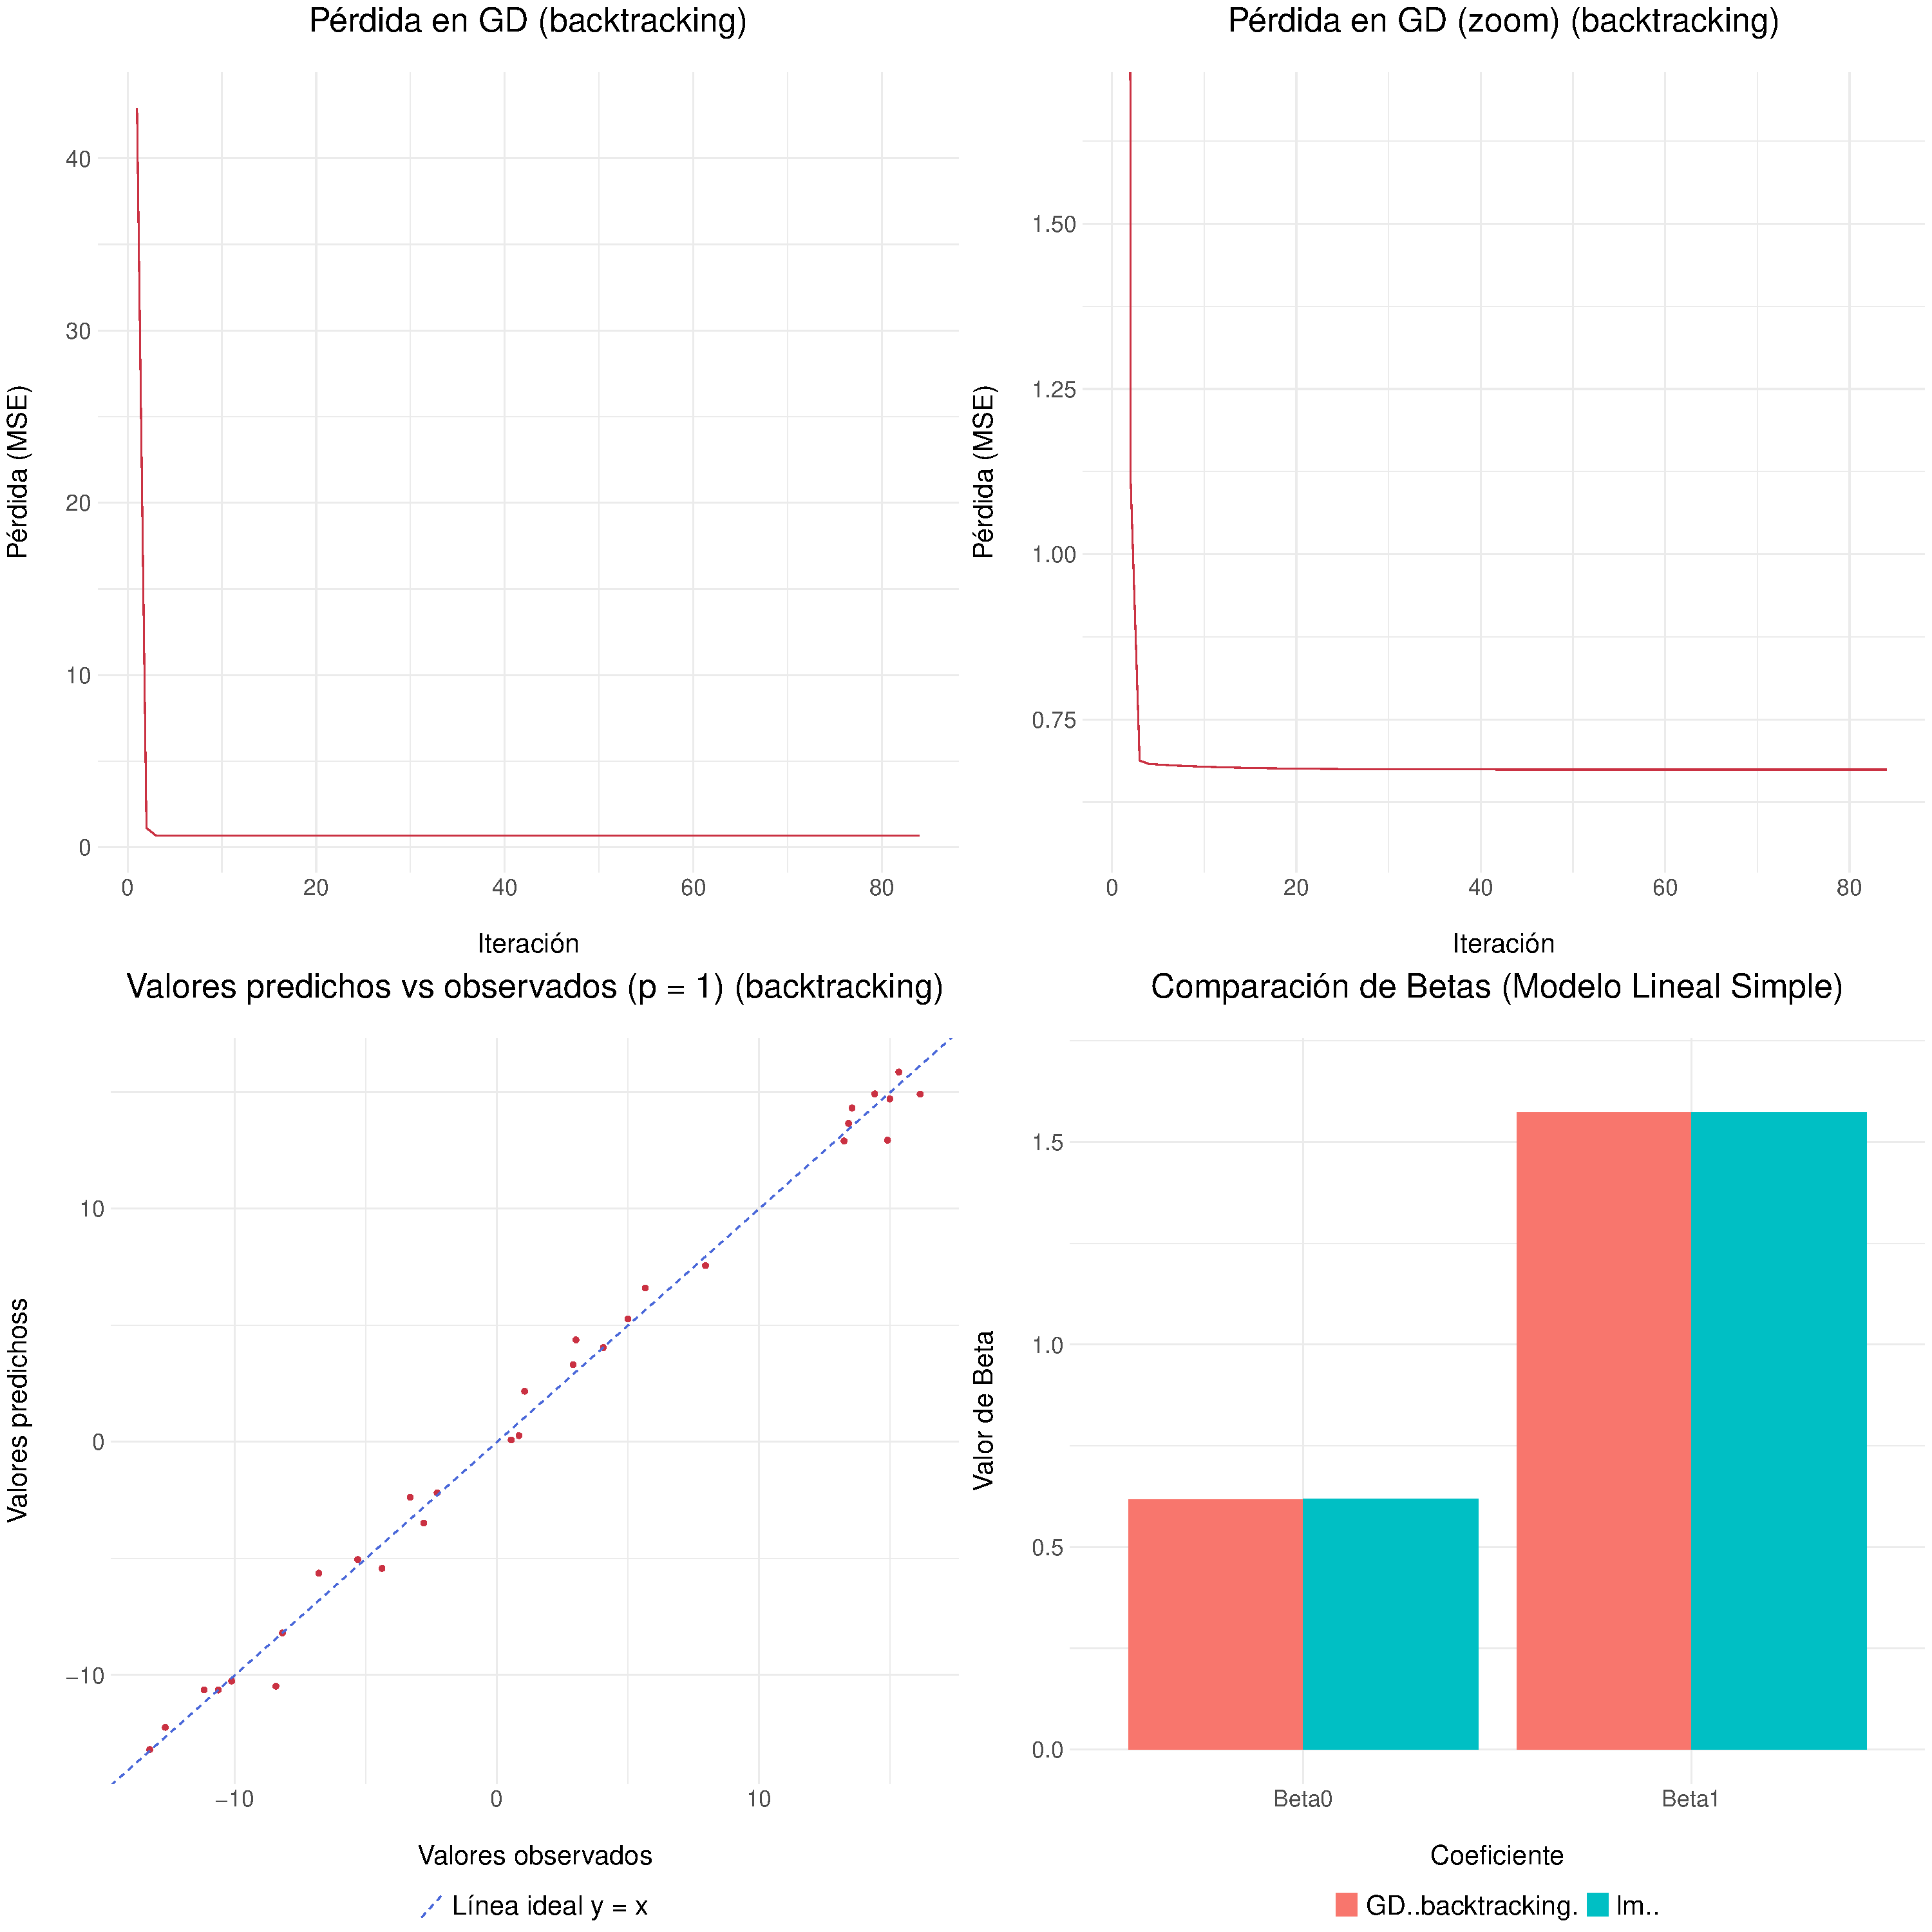
\includegraphics[width=0.8\textwidth]{fotos/plotmrs_pred.pdf}
\caption{Predicciones del modelo lineal simple haciendo uso de \textit{backtracking} con paso inicial $t=0.03$, empleando MSE como función de coste.}
\label{fig:11}
\end{figure}

Una vez analizado el comportamiento del modelo solo queda probarlo en datos que no haya visto y ver si se comporta bien. Se atenderá a las gráficas que muestran valores predichos frente a los observados, calculando el RSE y el $R^2$ para ver cómo de buena es la recta de pendiente unidad para describir la relación entre estas magnitudes, y la comparación de los coeficientes $\beta$. Para hacer predicciones solo se hará uso del modelo de GD con \textit{backtracking}. \\

En la figura \ref{fig:11} se ven los resultados antes mencionados. La estimación de los coeficientes es muy similar a la hecha con los datos de entrenamiento, dando simpre valores casi iguales a los dados por \texttt{lm()}. En cuanto a las predicciones, se ve que los valores caen en los alrededores la recta ideal $y=x$, siendo un buen ajuste visual. Si se acude de nuevo a la estadística $R^2$ y al RSE para ver cómo de buena es esta predicción numéricamente se tiene:
\begin{multicols}{2}
\begin{itemize}
\item RSE: $0.8351097$
\item $R^2$: $0.9925149$
\end{itemize}
\end{multicols}

El RSE es menor que en el entrenamiento, lo que indica una buena capacidad de extrapolación, y se mantiene un buen $R^2$, cercano a 1. 

\subsection{Modelo multilineal}

\subsubsection{Entrenamiento}

En la tabla \ref{tab:2} se muestran los resultados de todos los coeficientes estimados. Si se analiza con cuidado, se llega a que los resultados de los tres métodos son muy similares. Al disponer de tantos coeficientes, esta visualización de los datos no es la más cómoda, por lo que se grafican en la figura \ref{fig:2}, abajo a la derecha. Como ya se comentó, para un gran número de coeficientes el gráfico de barras no resulta lo más adecuado: aquí vemos los coeficientes estimados (por el método GD con \textit{backtracking}) frente a los estimados por el método \texttt{lm()}. Que los valores numéricos son extremadamente próximos se puede ver a simple vista, ya que los puntos caen sobre la recta ideal $y=x$. Esta representación facilita encontrar problemas con la estimación de algún coeficiente en específico (si fuese el caso).

\begin{table}[h]
    \resizebox{\textwidth}{!}{
    \centering
    \begin{tabular}{cccccccccccc}
    \hline
    \textbf{Método} & \textbf{Intercepto ($\beta_0$)} & $\boldsymbol{\beta}_1$ & $\boldsymbol{\beta}_2$ & $\boldsymbol{\beta}_3$ & $\boldsymbol{\beta}_4$ & $\boldsymbol{\beta}_5$ & $\boldsymbol{\beta}_6$ & $\boldsymbol{\beta}_7$ & $\boldsymbol{\beta}_8$ & $\boldsymbol{\beta}_9$ & $\boldsymbol{\beta}_{10}$  \\
    \hline
    Coeficientes GD (paso fijo) & $-3.2632605$ & $6.7557303$ & $-0.8420791$ & $8.6800341$ & $9.8218978$ & $-8.0734749$ & $1.5465260$ & $8.8582421$ & $2.0411180$ & $0.1446423$ & $10.1316270$ \\
    Coeficientes GD (backtracking) & $-3.2632817$ & $6.7557302$ & $-0.8420792$ & $8.6800338$ & $9.8218976$ & $-8.0734745$ & $1.5465254$ & $8.8582418$ & $2.0411178$ & $0.1446425$ & $10.1316268$ \\
    Coeficientes lm & $-3.2649436$ & $6.7557221$ & $-0.8420915$ & $8.6800064$ & $9.8218835$ & $-8.0734459$ & $1.5464835$ & $8.8582184$ & $2.0410969$ & $0.1446580$ & $10.1316126$ \\
    \hline
    \end{tabular}
    }
    \caption{Coeficientes estimados para el modelo de regresión multilineal durante el entrenamiento.}
    \label{tab:2}
\end{table}

Así como para la comparación de coeficientes solo se usan los dados por \textit{backtracking} y no por paso fijo, se hará lo mismo para la representación de la evolución de la pérdida y para la comparación de los valores predichos con los reales. En este caso, la única diferencia notoria son las iteraciones de cada uno: mientras que para GD con paso fijo, el mejor de los evaluados es un GD con $t = 10^{-5}$, que converge a las $391011$ iteraciones, el GD con \textit{backtracking}, comenzando en $t=0.01$, converge en solo $389$ iteraciones. \\

La novedad en la evolución de pérdida respecto al modelo más simple resulta evidente: al haber más iteraciones, la curva se suaviza en gran medida, parando en un MSE menor a $0.9$ en mil veces menos iteraciones que con paso fijo. \\

Una diferencia notoria respecto al modelo simple es la exactitud de las predicciones. Al representar los valores predichos frente a los observados (abajo a la izquierda), se ve que todos caen de forma perfecta sobre la recta ideal $y=x$. Como esta apreciación visual puede verse afectada por la escala de los ejes, se acude de nuevo a la estadística $R^2$ y al RSE para ver cómo de buena sería la recta de pendiente unidad para describir la relación entre estas magnitudes (se incluyen los resultados numéricos del GD con paso fijo, por comparar):
\begin{multicols}{2}
\begin{itemize}
\item RSE paso fijo: $0.9685707$ 
\item $R^2$ paso fijo: $0.9999513$ 
\item RSE \textit{backtracking}: $0.9685707$
\item $R^2$ \textit{backtracking}: $0.9999513$
\end{itemize}
\end{multicols}

De nuevo se tiene un $R^2$ cercano a 1, por lo que se afirma que la mayor parte de la variabilidad de estos datos queda completamente descrita por esta recta ideal $y=x$. Además, el RSE es incluso menor que en el caso de la regresión simple. Una desviación de $0.97$ para valores en un rango $[-300, 300]$ muestran un ajuste extremadamente bueno de los datos a esta recta. Todo esto, verifica la precisión de los valores predichos para este modelo multidimensional de 10 predictores.

\begin{figure}[H]
\centering
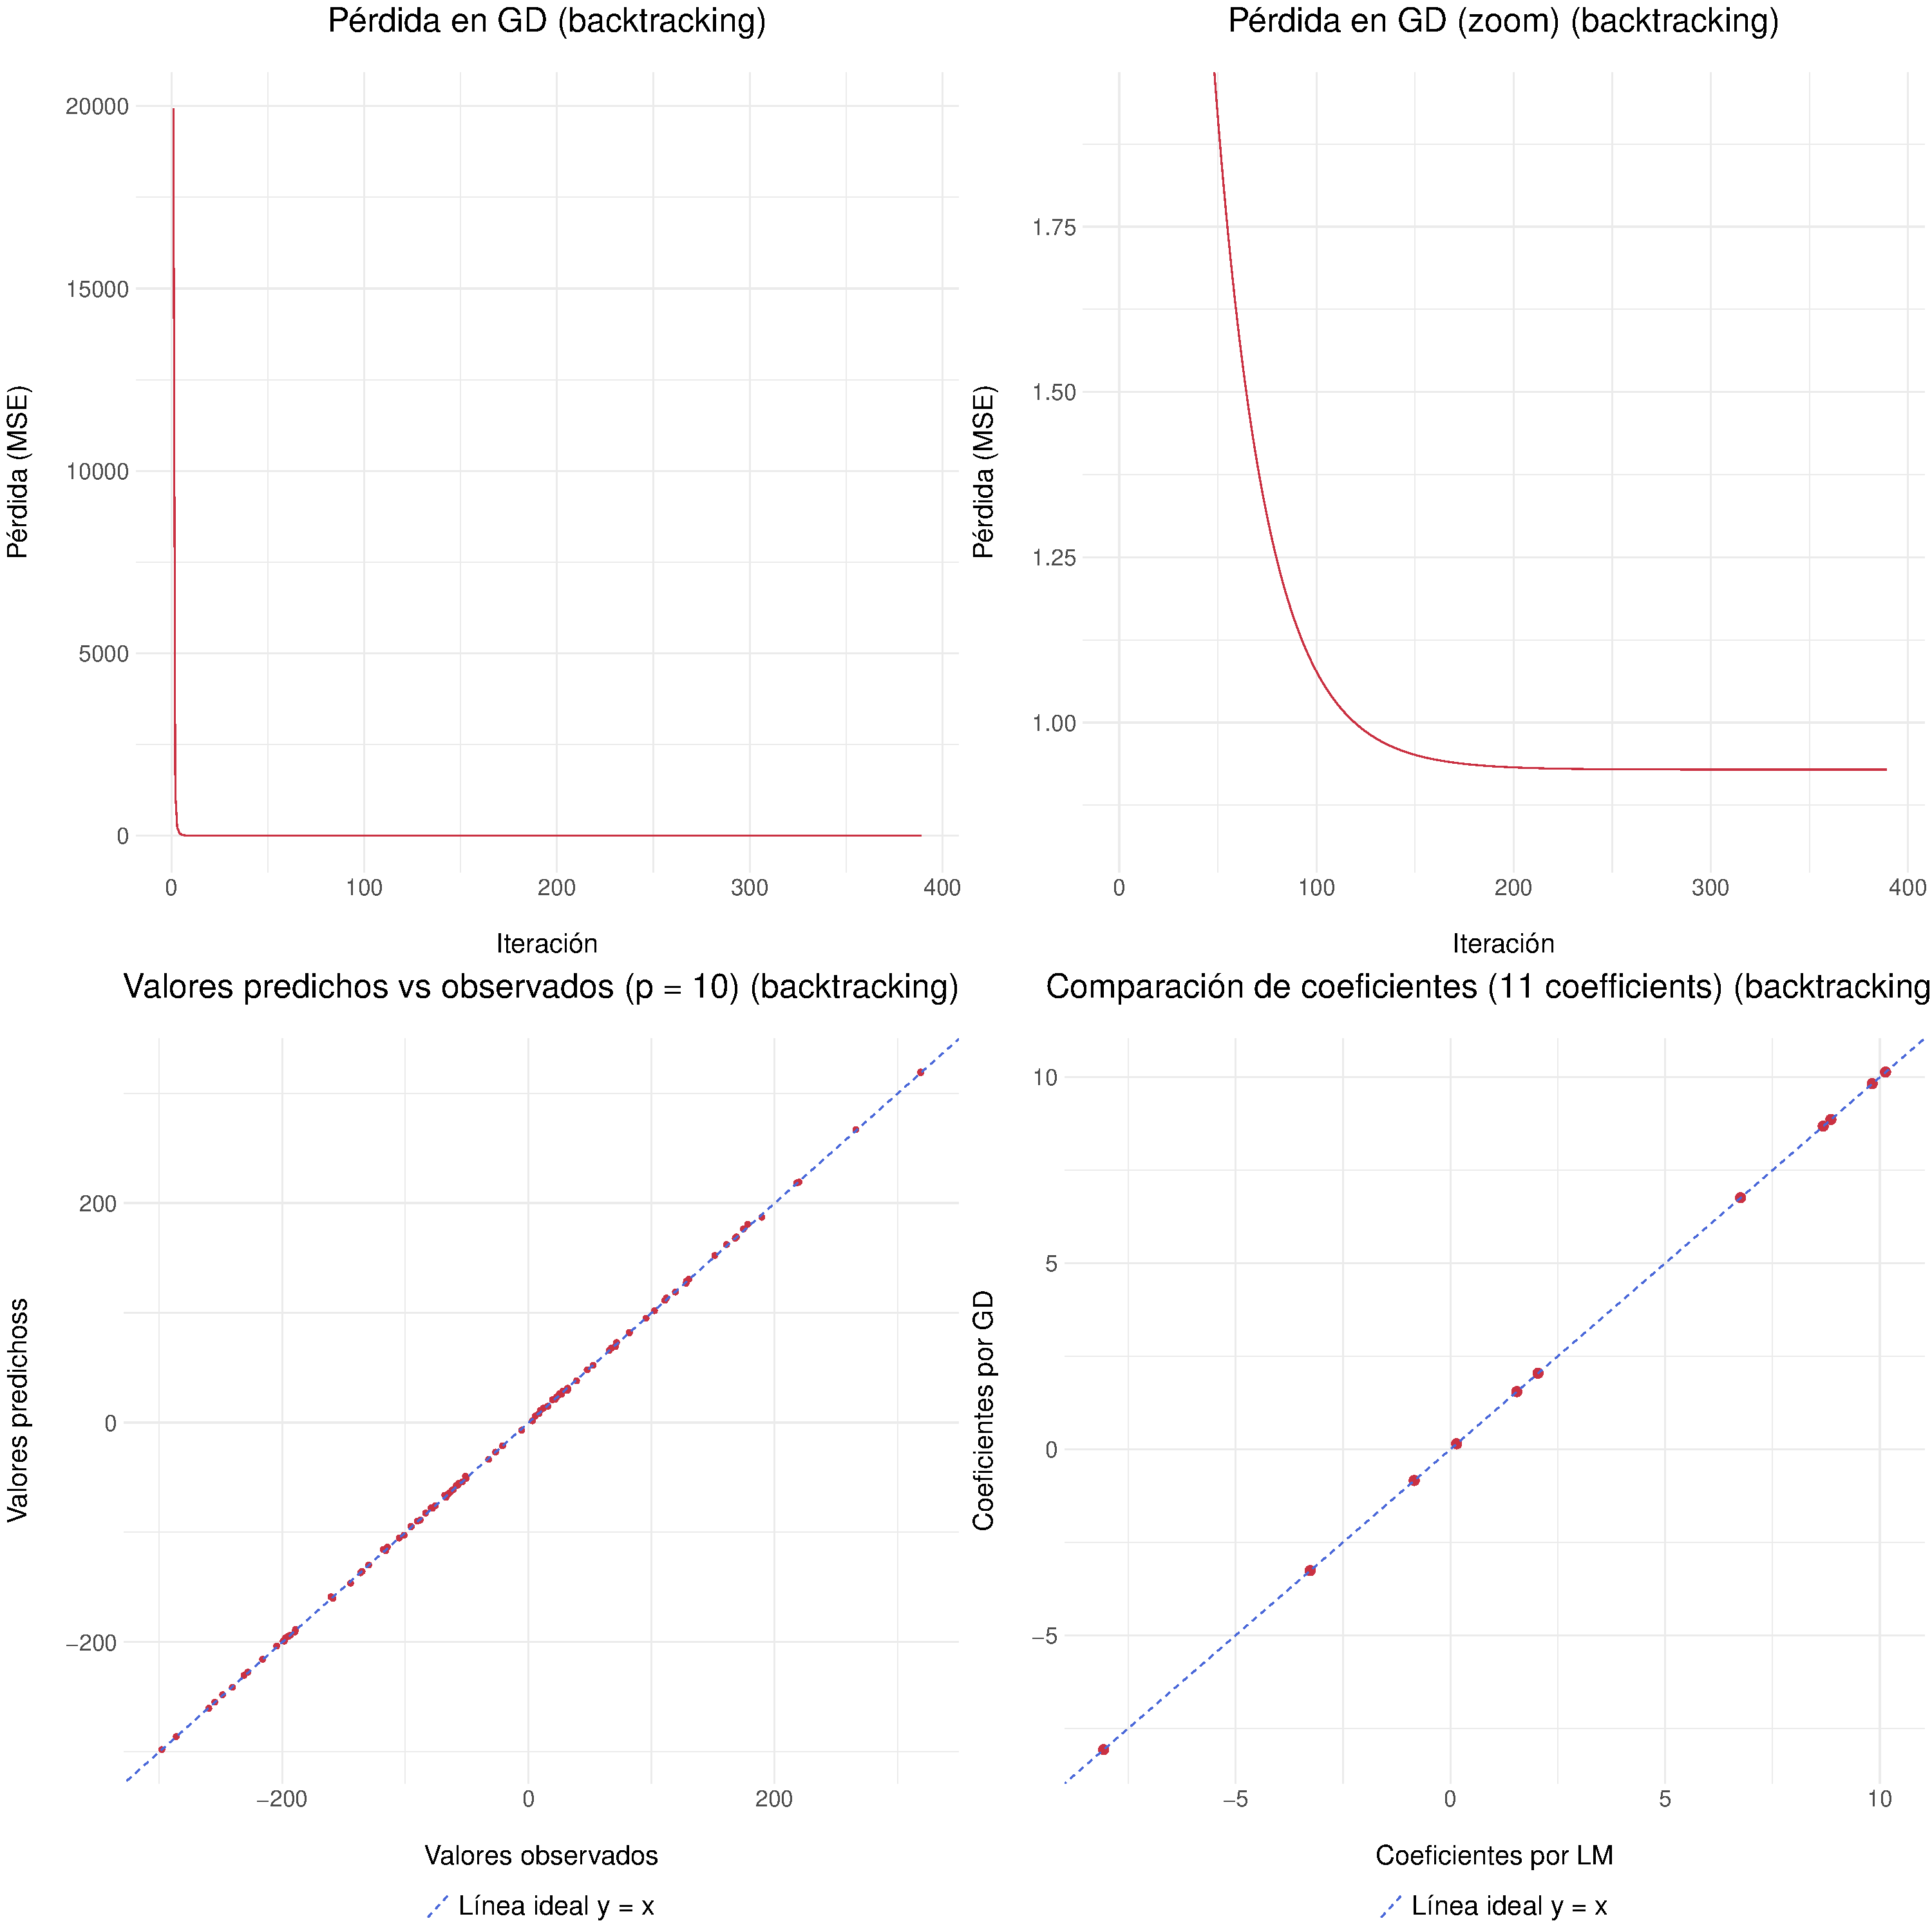
\includegraphics[width=\textwidth]{fotos/plot_multi.pdf}
\caption{Resultados de entrenamiento del modelo multilineal con $p=10$ haciendo uso de paso fijo y \textit{backtracking}, empleando MSE como función de coste.}
\label{fig:2}
\end{figure}

\subsubsection{Predicciones}

Aquí se tiene un análisis muy similar al anterior. En este caso, los coeficientes estimados por GD con \textit{backtracking} son prácticamente idénticos a los dados por \texttt{lm()}, al caer todos sobre la recta $y=x$. En cuanto a las predicciones, se tiene una mejora notable, al menos en lo visual, respecto al modelo simple: en este caso, los predicciones caen de forma casi perfecta sobre la recta ideal. Esto, como se comenta en el análisis del entrenamiento, puede estar sujeto a sesgo, debido a la escala de los valores. Para cuantificar esto con el RSE y el $R^2$:
\begin{multicols}{2}
\begin{itemize}
\item RSE: $0.8364551$ 
\item $R^2$: $0.999921$ 
\end{itemize}
\end{multicols}

La variabilidad de las predicciones queda casi perfectamente descrita por la recta ideal, sin embargo el RSE, pese a parecer menor que el del modelo simple (en predicciones) es muy similar. No obstante, resulta menor que el mostrado con los datos de entrenamiento para este modelo, por lo que resultan buenas predicciones.

\begin{figure}[H]
\centering
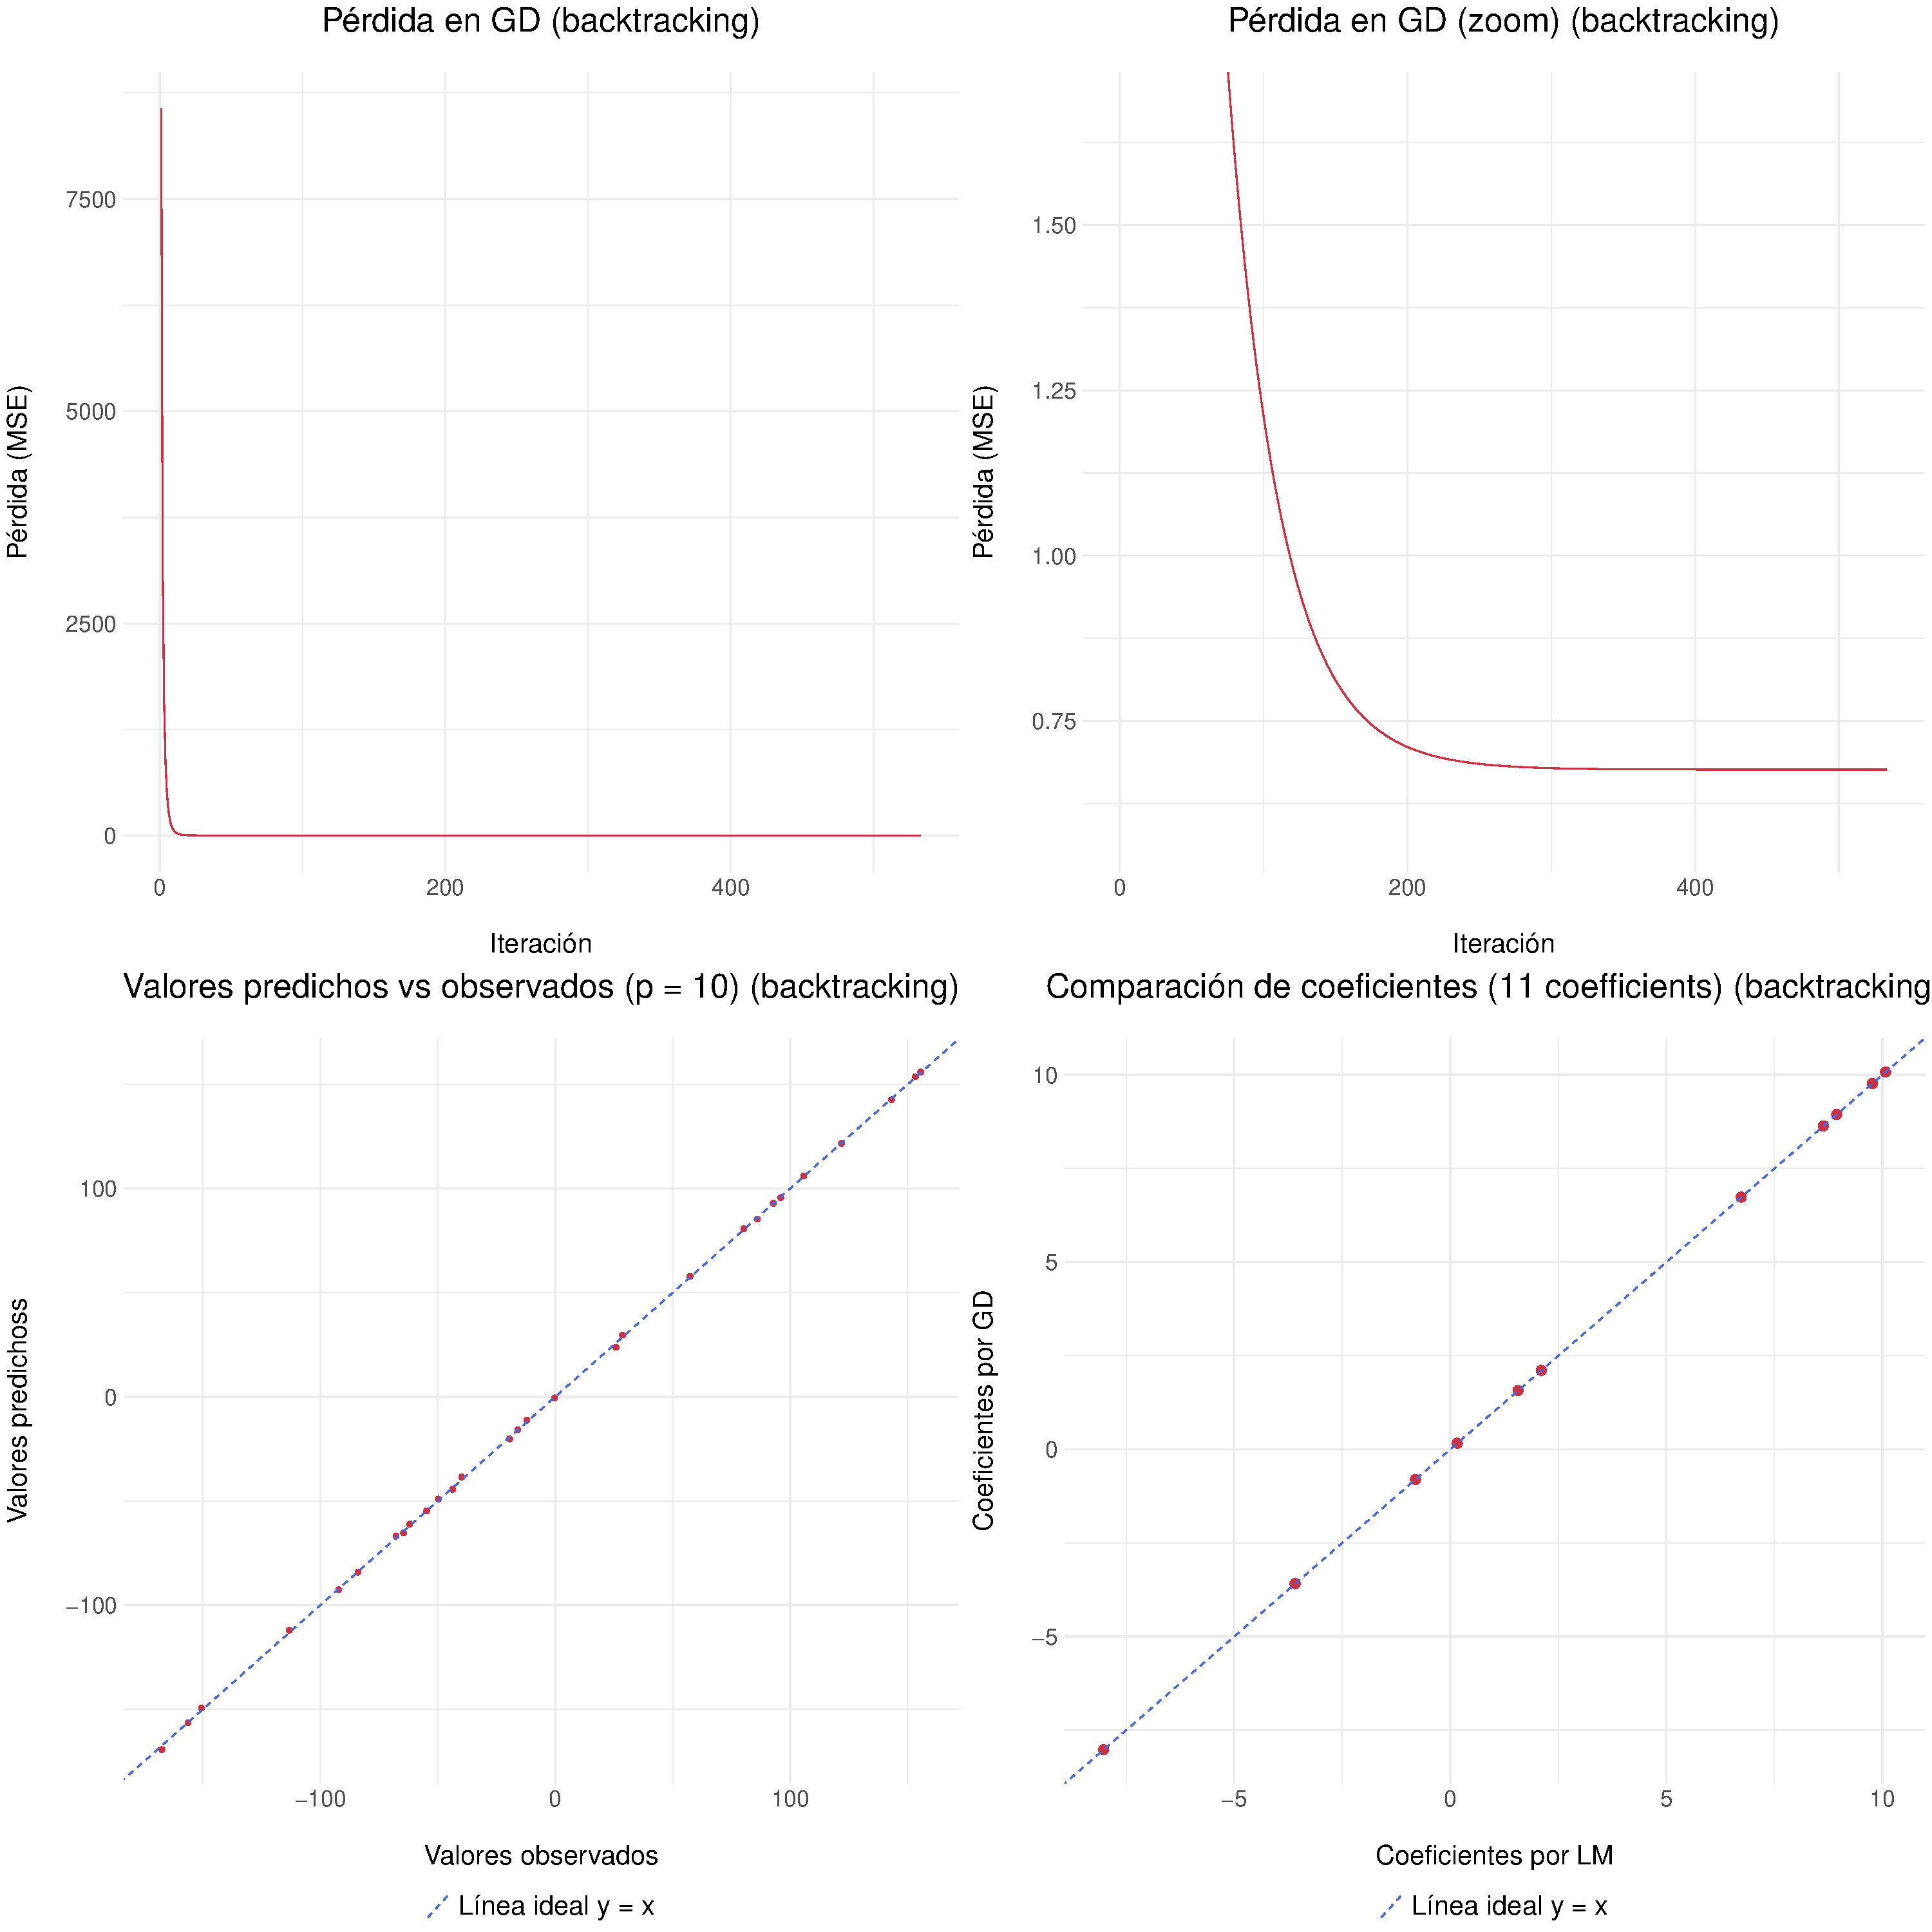
\includegraphics[width=0.8\textwidth]{fotos/plot_multi_pred.pdf}
\caption{Predicciones del modelo multilineal con $p=10$ haciendo uso de \textit{backtracking} con paso inicial $t = 0.01$, empleando MSE como función de coste.}
\label{fig:22}
\end{figure}


\subsection{Modelo cuadrático}

\subsubsection{Entrenamiento}

Este caso supone una complicación sobre el modelo lineal, al añadir un término cuadrático. Sin embargo, en cuanto a la estimación de parámetros, tendremos un problema de menor calibre que el modelo multidimensional antes caracterizado. \\

El mejor modelo de GD con paso fijo usó un $t = 10^{-5}$ y $596557$ iteraciones para converger, mientras que con \textit{backtracking} y un paso inicial de $10^{-3}$, el algoritmo solo necesita $7448$ iteraciones. \\

Como en los ejemplos anteriores, se muestra en la tabla \ref{tab:3} la comparativa numérica de los coeficientes estimados. Al ser pocos, tanto la tabla como el gráfico de barras de la figura \ref{fig:3} (abajo a la derecha), son visualizaciones óptimas de estos resultados, aunque la numérica permite hacer una distinción más clara. Al tener estimaciones muy similares que conducirán a resultados muy próximos, empleamos el mismo recurso que en el apartado anterior, y se muestran los resultados del GD con \textit{backtracking}. 

\begin{table}[h]
    \centering
    \resizebox{0.9\textwidth}{!}{
    \begin{tabular}{cccc}
    \hline
    \textbf{Método} & \textbf{Término independiente ($\beta_0$)} & \textbf{Término lineal ($\beta_1$)} & \textbf{Término cuadrático ($\beta_2$)} \\
    \hline
    Coeficientes GD (paso fijo) & $-1.441886$ & $1.749778$ & $-0.5423135$ \\
    Coeficientes GD (backtracking) & $-1.442155$ & $1.749779$ & $-0.5423079$ \\
    Coeficientes lm & $-1.444952$ & $1.749790$ & $-0.5422550$ \\
    \hline
    \end{tabular}
    }
    \caption{Coeficientes estimados para el modelo de regresión cuadrático  durante el entrenamiento.}
    \label{tab:3}
\end{table}

\begin{figure}[H]
\centering
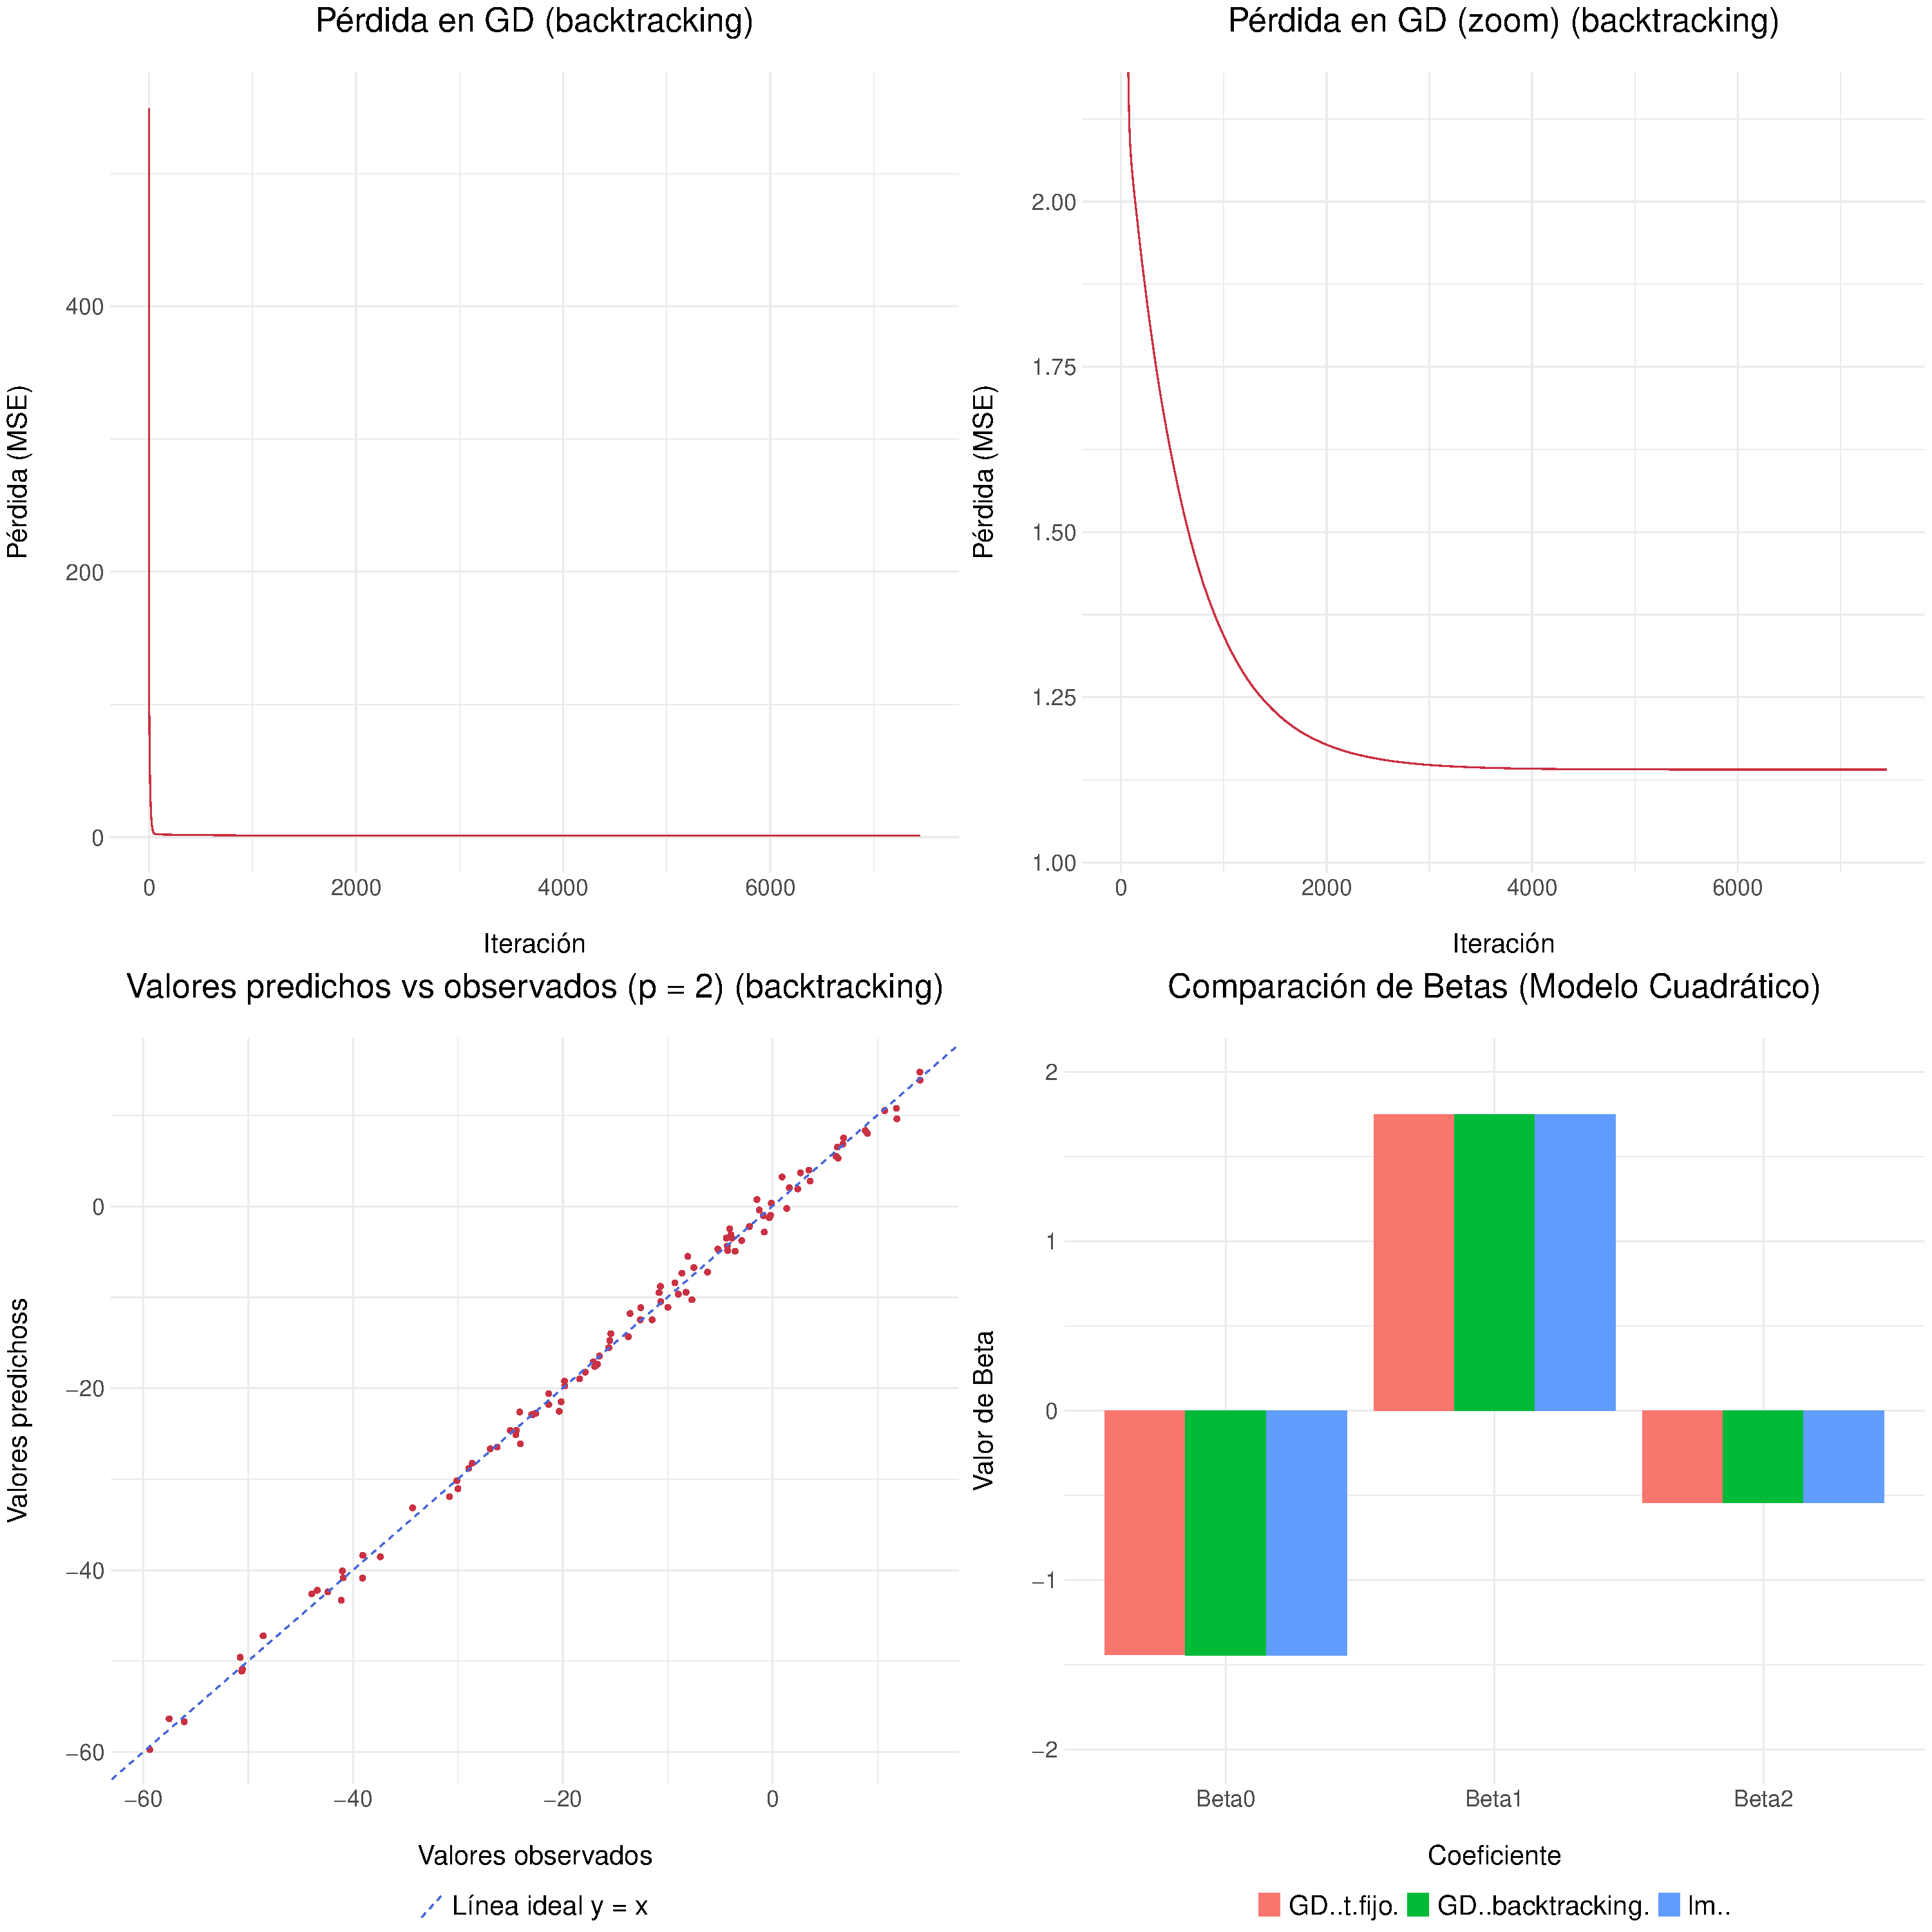
\includegraphics[width=\textwidth]{fotos/plot_cuad.pdf}
\caption{Resultados de entrenamiento del modelo cuadrático con $p=2$ haciendo uso de paso fijo y \textit{backtracking}, empleando MSE como función de coste.}
\label{fig:3}
\end{figure}

En este caso, el algoritmo converge en un MSE ligeramente superior a 1, lo que indica un resultado menos preciso. Esto se puede ver también en la comparativa entre valores predichos y observados: como ocurría en el caso del modelo lineal, los valores caen alrededor de la recta $y=x$, no sobre la misma como en el modelo multilineal. El RSE y el $R^2$ permitirán conocer la proximidad de estos datos a la recta ideal
\begin{multicols}{2}
\begin{itemize}
\item RSE paso fijo: $1.073384$ 
\item $R^2$ paso fijo: $0.9963831$ 
\item RSE \textit{backtracking}: $1.073384$
\item $R^2$ \textit{backtracking}: $0.9963831$
\end{itemize}
\end{multicols}

Si bien el $R^2$ indica que la variabilidad queda bien descrita por la recta, se tiene un RSE mayor a 1, lo cual solo ocurrió con el modelo simple. Considerando el rango de valores, no resulta una desviación preocupante, pero si que es destacable. Al aumentar la flexibilidad del modelo, se puede caer en problemas de \textit{overfitting}. \\

Al tratar con dos predictores, es posible una visualización en 3D de las superficies de regresión, para comparar las obtenidas por GD con las obtenidas por \texttt{lm()}. En la figura \ref{fig:4} se muestran estas superficies, donde se ve que son prácticamente idénticas al solaparse, lo mismo que ocurrió en el caso del modelo simple con las rectas de regresión.

\begin{figure}[H]
\centering

\includegraphics[width=\textwidth]{fotos/sup.png}
\caption{Superficies de regresión sobre los datos de entrenamiento para el modelo cuadrático calculadas por \texttt{lm()} (en azul) y por GD con \textit{backtracking}, empleando MSE como función de coste (en rojo).}
\label{fig:4}
\end{figure}

\subsubsection{Predicciones}

\begin{figure}[H]
\centering
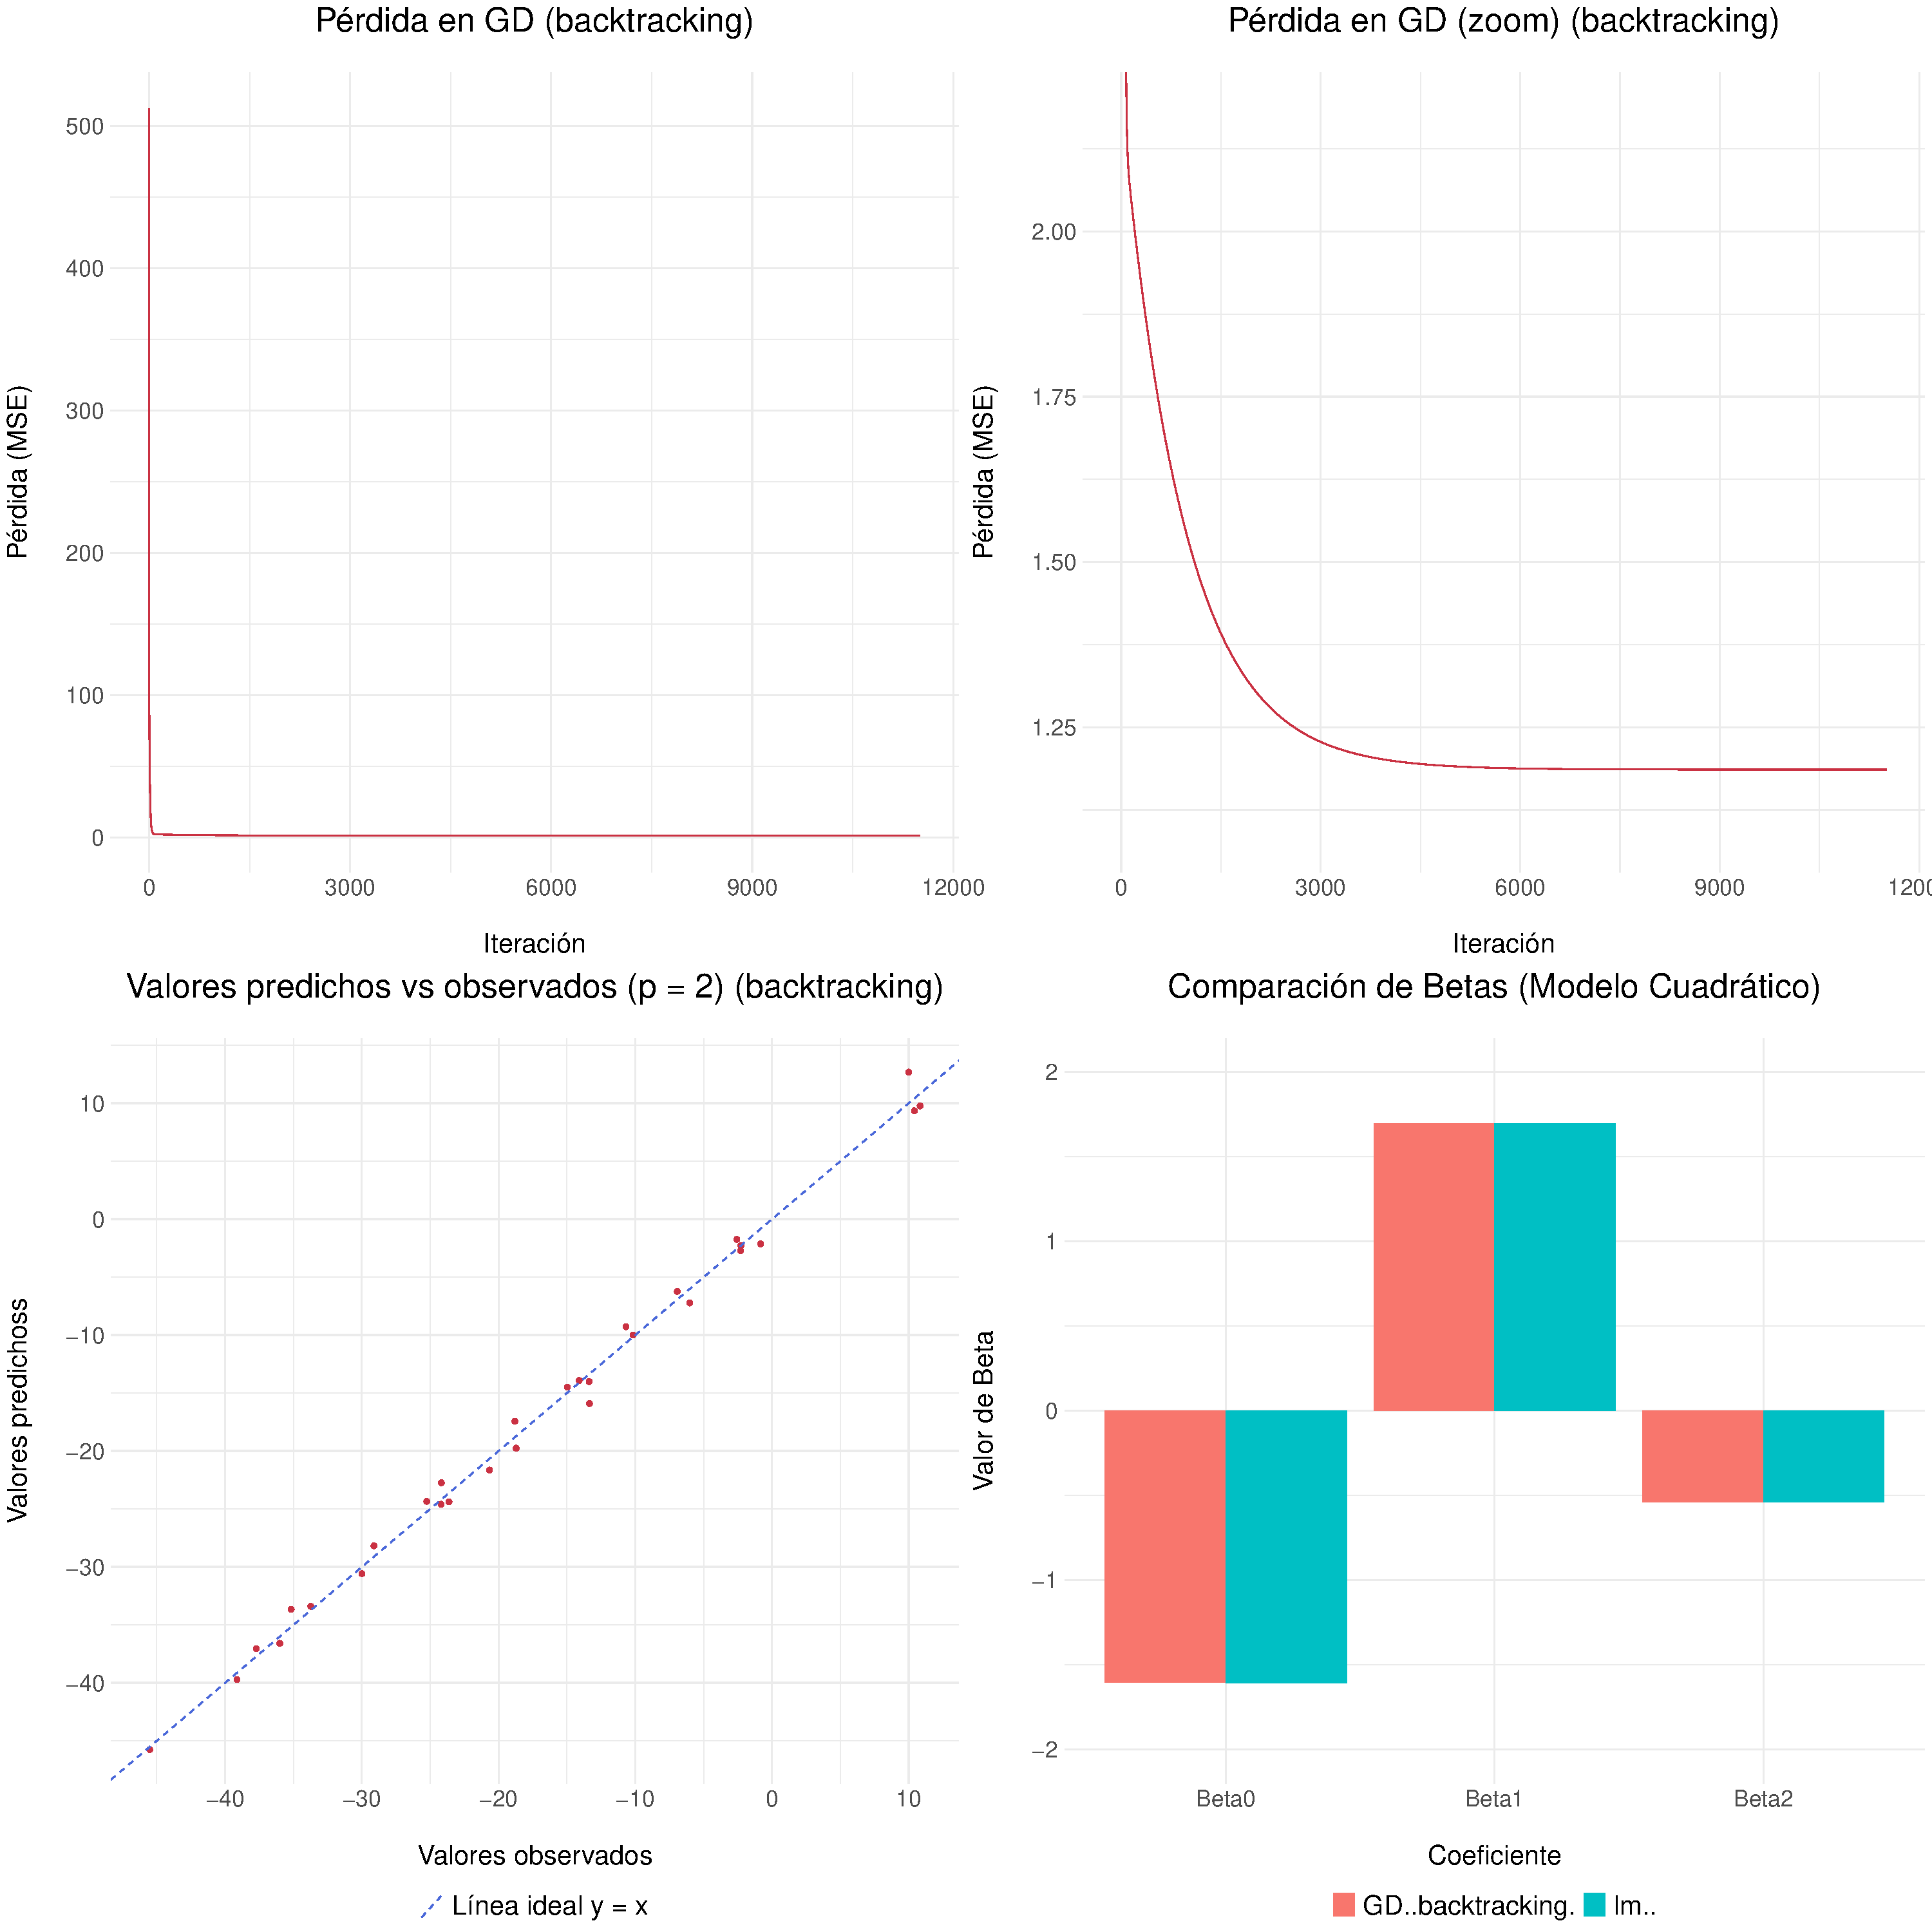
\includegraphics[width=0.8\textwidth]{fotos/plot_cuad_pred.pdf}
\caption{Predicciones del modelo cuadrático con $p=2$ haciendo uso de \textit{backtracking} con paso inicial $t = 10^{-3}$, empleando MSE como función de coste.}
\label{fig:33}
\end{figure}

En el caso del modelo cuadrático, se ve un comportamiento muy similar entre el conjunto de entrenamiento y el de \textit{test}: los coeficientes estimados son prácticamente idénticos, y las predicciones caen alrededor de la recta ideal, pero sin grandes desviaciones. Para dar una medida numérica, se recurre de nuevo al RSE y al $R^2$:
\begin{multicols}{2}
\begin{itemize}
\item RSE: $1.107571$
\item $R^2$: $0.994737$
\end{itemize}
\end{multicols}

El $R^2$ indica que la variabilidad de los resultados predichos frente a los reales queda bien descrita por la recta ideal. El RSE tiene un valor muy pequeño si se considera el rango de valores sobre el que se mueven las predicciones, pero resulta peor que en el caso de los datos de entrenamiento. Esto indica una peor actuación del modelo cuadrático en los datos de \textit{test} respecto a los de entrenamiento, y un posible indicio de \textit{overfitting}.

\section{Conclusiones}

Se trataba de resolver un problema de regresión con el método de descenso de gradiente (GD). Concretamente, se estudiaron tres modelos distintos: un modelo lineal simple, un modelo multilineal de $p = 10$ y un modelo cuadrático. Para cada uno de ellos, se compararon los resultados obtenidos por GD (con paso fijo y \textit{backtracking}) con los obtenidos por el método \texttt{lm()}, que son los ideales. \\

En el caso de los dos modelos lineales, se realiza un buen entrenamiento y la actuación sobre los datos de \textit{test} es excelente, logrando incluso reducir el RSE mostrado durante el proceso de entrenamiento. Aumentar el número de predictores permitió dar más información de aprendizaje el algoritmo para que capturara mejor la relación entre las variables, lo que permitió dar resultados más precisos en el caso multilineal. Sin embargo, aumentar la flexibilidad del modelo a uno cuadrático supuso un RSE mayor en los datos de \textit{test} que en los de entrenamiento, lo que puede ser un indicio de \textit{overfitting}. No obstante, la diferencia es pequeña, de modo que no se tiene un problema real para la magnitud de esta muestra. \\

Se ha podido comprobar que el uso de \textit{backtracking} es más eficiente que el uso de un paso fijo, y que los resultados obtenidos por GD son muy similares a los obtenidos por \texttt{lm()}, lo que indica que el algoritmo de descenso de gradiente implementado es correcto. Para finalizar, también se pudo comprobar el hecho de que aumentar la flexibilidad del modelo puede llevar a problemas de \textit{overfitting}.

\end{document}
